\documentclass[10pt,twocolumn,letterpaper]{article}

\usepackage{cvpr}
\usepackage{times}
\usepackage{epsfig}
\usepackage{graphicx}
\usepackage{amsmath}
\usepackage{amssymb}

% Include other packages here, before hyperref.

% If you comment hyperref and then uncomment it, you should delete
% egpaper.aux before re-running latex.  (Or just hit 'q' on the first latex
% run, let it finish, and you should be clear).
\usepackage[pagebackref=true,breaklinks=true,letterpaper=true,colorlinks,bookmarks=false]{hyperref}

\cvprfinalcopy % *** Uncomment this line for the final submission

\def\cvprPaperID{****} % *** Enter the CVPR Paper ID here
\def\httilde{\mbox{\tt\raisebox{-.5ex}{\symbol{126}}}}

% Pages are numbered in submission mode, and unnumbered in camera-ready
\ifcvprfinal\pagestyle{empty}\fi
\begin{document}

%%%%%%%%% TITLE
% \title{Project Report : CS 4803/7643 Spring 2020 \\ 
\title{YouTube Link Prediction using Graph Neural Nets}

\author{David Gong\\
Georgia Institute of Technology\\
Atlanta, GA, USA\\
{\tt\small davidcgong@gatech.edu}
% For a paper whose authors are all at the same institution,
% omit the following lines up until the closing ``}''.
% Additional authors and addresses can be added with ``\and'',
% just like the second author.
% To save space, use either the email address or home page, not both
\and
Reagan Kan\\
Georgia Institute of Technology\\
Atlanta, GA, USA\\
{\tt\small rkan3@gatech.edu}
\and
Sreyans Sipani\\
Georgia Institute of Technology\\
Atlanta, GA, USA\\
{\tt\small ssipani6@gatech.edu}
\and
Jeremy Kwok\\
Georgia Institute of Technology\\
Atlanta, GA, USA\\
{\tt\small secondauthor@i2.org}

}

\maketitle
%\thispagestyle{empty}

%%%%%%%%% ABSTRACT
\begin{abstract}
    In this paper, we explored the possibilities of applying a graph neural network (GNN) to produce related YouTube videos for newly generated videos using link prediction. We conducted representation learning for our dataset by applying graph embedding techniques such as node2vec and spectral embedding. These new inputs from the embeddings feed to a GNN for calculations. We also investigated a novel method of combining both SEAL and spectral embedding for link prediction. The results and analyses indicate an alternative approach for video recommendation tasks, which is both scalable and accurate. We find that GNNs can be further explored for building video recommendation systems.
%   The ABSTRACT is to be in fully-justified italicized text, at the top
%   of the left-hand column, below the author and affiliation
%   information. Use the word ``Abstract'' as the title, in 12-point
%   Times, boldface type, centered relative to the column, initially
%   capitalized. The abstract is to be in 10-point, single-spaced type.
%   Leave two blank lines after the Abstract, then begin the main text.
%   Look at previous CVPR abstracts to get a feel for style and length. 
%   The abstract section should contain a brief summary of your work that
%   includes the problem statement, proposed solution and results.
\end{abstract}

%%%%%%%%% BODY TEXT
\section{Introduction}

% \textbf{(5 points) What did you try to do? What problem did you try to solve? Articulate your objectives using absolutely no jargon.} 

On YouTube, hours of content is being uploaded every second \cite{youtube-original}. This generates a rich network of new data that is being added to the back-end servers at any given time. In the context of this paper, we will think of this network as a graph. This is important because each video, which represents a node, will need to generate directed edges to other nodes (other videos) in order for there to be recommended videos. We consider the following problem.

\begin{enumerate}
    \item Given a set of nodes and a query node, utilize link prediction / GNN to accurately predict related IDs for the query node.
\end{enumerate}

% \textbf{(5 points) Who cares? If you are successful, what difference will it make?} 

The results gathered from this project introduce an alternative other than deep neural networks for YouTube video recommendation. Further research into this topic from previous papers introduced practical applications for social networks, leading us to believe that the same interpretations could be said for video based platforms like YouTube and other various, cutting-edge applications such as cancer detection. We now discuss papers that relate to the research at hand.


\section{Related works}
% \textbf{(5 points) How is it done today, and what are the limits of current practice?}

Currently, the approach that YouTube utilizes for recommending videos is detailed by the paper "Deep Neural Networks for YouTube Recommendations" which was written by Paul Covington, Jay Adams, and Emre Sargin in 2016. The first layer consists of candidate generation, in which a deep learning neural network determines hundreds of related content. The second and final layer consists of utilizing user activity, video characteristics, and other candidate traits to further filter the related content by ranking them --- providing dozens of personalized recommendations for the user based on the video that is viewed \cite{youtube-original}.

As far as the limits of current practice, this seems to be a generally accurate and encompassing approach to recommend videos to users. However, one can make the argument that as the number of videos grows, so does the training time due to the model being all encompassing. Being able to think about the collection of videos as a network allows us to investigate and compare how a graph neural network and other graph-dependent techniques such as SEAL can be applied rather than a deep neural network. While not investigated in this paper, we also believe that a varied implementation of the PageRank algorithm could also lead to positive results.

Other papers such as \textit{The link prediction problem for social networks} by David Liben-Nowell and Jon Kleinberg in 2013 indicate various link prediction algorithms (Adamic-Adar, Jaccard's coefficient, common neighbors, etc.) that have been used, along with performance comparisons. \cite{link-prediction-social-network} We similarly compare these within the paper, and then lastly compare the results for our GNN specifically for our problem.

% Given the nature of YouTube’s current recommendation algorithm as specified by the 2016 paper "Deep Neural Networks for YouTube Recommendations" by Covington, Adams, and Sargin \cite{youtube-original}, the current algorithm does not utilize GNNs. As can be seen in \cite{youtube-original}, YouTube’s current algorithm devises a separate recommendation system architecture that involves generating hundreds of candidate videos, and then utilizing user activity, video features, and other candidate sources to rank these videos. This eventually reduces the amount of ranked videos to just dozens, which are then listed as related videos. There seems to be relatively little limits to current practice, though having both models perform calculations and analyze interactions with A/B testing could be beneficial.
\section{Dataset}
% \textbf{(5 points) What data did you use? Provide details about your data, specifically choose the most important aspects of your data mentioned \href{https://arxiv.org/abs/1803.09010}{here}. You don’t have to choose all of them, just the most relevant.}

For this study, we used the data set \href{https://netsg.cs.sfu.ca/youtubedata/}{here} \cite{4539688}, which was crawled in 2007 and 2008. According to Cheng, Dale, and Liu, they considered all YouTube videos to form a directed graph with each other. Each video represents a node within the graph, and for each video, if there is a video $b$ in the related video list of a video $a$, then there is a directed edge from the node $a$ to node $b$. There can only be 20 connections at once for our dataset, but the main purpose of us utilizing this dataset is so that we can quickly generate embeddings and clustering tasks within the context of utilizing GNNs. In addition, there are 3 depths of video data labelled for each of the dates within the data set. We chose the .txt file which had video data with 3 depths for our analyses, specifically from the .zip file named 080327.zip. The crawled data is labelled in the following table as can also be seen in \cite{4539688}:

\begin{center}
\begin{tabular}{|c|c|}
\hline
 video ID & \verb string \\
 uploader & \verb string \\
 age & \verb integer \\
 category & \verb string \\
 length & \verb int \\
 views & \verb int \\
 rate & \verb float \\
 ratings & \verb float \\
 comments & \verb int \\
 related IDs & \verb string \\
 \hline
\end{tabular}\\
\end{center} 

Some further analysis on the graph structure shows that the maximum degree of a node is close to 300 and there are only a few vertices with degree in the order $10^2$. 
For our proposed algorithm, we did not exclude any of the variables for our deep learning neural net. Our output variable is the related IDs field.

\begin{figure}[t]
\begin{center}
   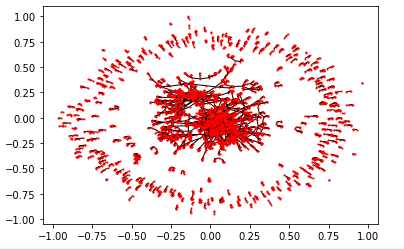
\includegraphics[width=1\linewidth]{latex/images/graph-viz.PNG}
\end{center}
   \caption{Visualization of the graph network for the extracted YouTube dataset.}
\label{fig:long}
\label{fig:onecol}
\end{figure}
%-------------------------------------------------------------------------
%------------------------------------------------------------------------
\section{Approach}
We first processed the data from the website by converting it to an adjacency matrix. In addition, due to computational constraints, we restricted the amount of connections that we used to train our model. For each node that we parsed per line, we grabbed all of its neighbors and repeated this same step for a limited amount of iterations.

After the adjacency matrix was created, we ran our embeddings and link prediction baseline algorithms on it.


%-------------------------------------------------------------------------
% %------------------------------------------------------------------------
% \section{Embeddings}

% \textbf{(10 points) What did you do exactly? How did you solve the problem? Why did you think it would be successful? Is anything new in your approach?} 

In order to effectively utilize GNNs, we first needed to generate embeddings for the dataset to simplify our downstream deep learning neural net classification task. Excluding the action of utilizing feature learning in a separate module often leads to low performance and accuracy. We explored two different methods of graph embeddings, then compared separate link prediction methods for the problem. 

As a novelty, we also combined spectral embedding with the SEAL (Subgraphs, Embeddings, and Attributes for Link Prediction) framework to combine subgraph evaluation and factoring in node separation distance importance.

\subsection{node2vec}

We used node2vec, which was introduced by Grover and Leskovec in 2016 \cite{node2vec}. node2vec is a semi-supervised algorithm that is used for representation learning on graphs, where continuous feature representations can be learned for the nodes - resulting in various uses for machine learning or deep learning tasks \cite{node2vec}. Nodes can be mapped to a low-dimensional space of features that maximises the likelihood of preserving network neighbour of nodes. Using a Skip-gram model to networks to define a objective function over it's neighbours. We construct the neighbourhood using random walks and compute gradients for our objective function. We use SGD for optimisation. This helps our case of predicting related videos not connected by an edge.

\subsection{Spectral embedding}

In addition to node2vec, we also utilized spectral embedding, specifically from the scikit-learn library. The process is as follows: \cite{spectral-embed}

\begin{itemize}
    \item Data sample is projected on the first eigenvectors of the graph Laplacian.
    \item The adjacency matrix is used to compute a graph Laplacian that has been normalized which has a spectrum that can interpret the minimum number of cuts necessary to split the graph into comparably sized components.
\end{itemize}

According to scikit-learn's documentation, Laplacian Eigenmaps is the true algorithm that is implemented for spectral embedding.

\subsection{Variational Graph Auto-Encoder}

Here we pass the adjacency matrix and features through an auto-encoder to output a reconstructed adjacency matrix used for link prediction. We calculate the hidden layer using a graph convolution layer as follows - 
\[
H = ReLU(A*F*W_1)
\]
where A is the adjacency matrix, F is the node features and W is the weights of the layer. We then use the hidden layer and the adjacency matrix to calculate the mean node embeddings and the standard deviation using graph convolution layers as well. Then the node embeddings are sampled using a normal distribution using the above 2 parameters.
\[
\mu = A*H*W^\mu_2
\]
\[
\sigma = A*H*W^\sigma_2
\]
\[
Z \sim N(\mu, \sigma)
\]
All the above layers use dropout. We finally reconstruct the adjacency matrix by computing an inner product on Z - 
\[
A' = Z*Z^T
\]
The training is done using cross entropy loss and updation based on Adam optimization. The above implementation is based on \cite{lucas-hu}.

\subsection{Problems anticipated}

We anticipated that no embeddings or versions of representation learning would lead to a significant decrease in performance. We expand upon this in further detail in later sections.
The graph auto-encoder takes a very long running time for adjacency matrix with nodes in the order of $10^4$ on a single CPU. Therefore the later experiments are performed on carefully chosen subgraphs / subset of nodes.

% \textbf{(5 points) What problems did you anticipate? What problems did you encounter? Did the very first thing you tried work?}


% \textbf{Important: Mention any code repositories (with citations) or other sources that you used, and specifically what changes you made to them for your project. }

\section{Experimentation \& Results}

After applying the embedding algorithms, we sought to compare the accuracies and performance of various link prediction baseline methods. For this portion of our project, we utilized the Github repository from \href{https://github.com/lucashu1/link-prediction}{github.com/lucashu1/link-prediction} \cite{lucas-hu}, namely making changes to the link prediction baseline Jupyter notebook by adding additional algorithms such as RA and adapting the code to Python 3 and utilizing NetworkX, a library that is used to create, manipulate, and structure complex networks. We additionally included a visualization of the node graph in Figure 1. We also augment the existing SEAL framework \href{https://github.com/muhanzhang/SEAL}{code} \cite{SEAL} by adding new embedding options, namely, spectral embedding and a hybrid node2vec and spectral embedding.

% \subsection{Common neighbors}

\subsection{Node neighborhoods (low-order heuristics)}

Within the context of link prediction, node neighborhood-based methods have been gaining popularity in use due to their simplicity and effectiveness. We explored the performances and implications between Adamic-Adar, Jaccard's coefficient, preferential attachment, and resource allocation. For this portion, we examined ROC curves and AP (average precision).  We first explain the concepts behind the baseline algorithms that were used / excluded from this project.

One popular method that we chose to exclude was Common Neighbors (CN), which is a relatively straightforward algorithm which scores by determining the number of neighbors that a node $x$ and a node $y$ have in common. \cite{link-prediction-social-network}

\[
score(x, y) = |\Gamma(x) \cap \Gamma(y)| 
\]

Common Neighbors are often combined with either computing the ratio of within and inter-cluster common neighbors of node pairs as was done by Valverde-Rebaza and Lopes \cite{within-cluster-common-neighbor} or through utilizing community information \cite{community-common-neighbor}. However, communities and clusters need to be defined and generated, and there is not enough reliable user data to construct accurate, disparate groups - thus the reason for CN's exclusion.

Jaccard's coefficient can be computed as follows \cite{link-prediction-social-network}:

\[
score(x, y) = \frac{|\Gamma(x) \cap \Gamma(y)| }{|\Gamma(x) \cup \Gamma(y)| }
\]

The idea behind Jaccard's coefficient is that it measures the probability that both x and y shares a similar feature $f$ which is randomly selected. \cite{link-prediction-social-network}.


Adamic-Adar is a common second order heuristic method for link prediction. The general notion behind this method is that sparse nodes should be weighted strongly because an edge between sparse nodes constitute more significance as opposed to a node with more edges. \cite{link-prediction-social-network} 


\[
    A(x, y) = \displaystyle\sum_{z \in N(x) \cap N(y)}^{} \frac{1}{log|N(z)|} 
\]

, where $N(z)$ is the set of nodes adjacent to $z$. \cite{link-prediction-social-network}

Preferential attachment operates on the premise that the probability that a new edge involves node $u$ is proportional to $|\Gamma(u)|$, which is the current number of neighbors of u. The equation is as follows:   

\[
    |\Gamma(u)|\cdot|\Gamma(v)|
\]

Lastly, we also analyzed resource allocation, which is defined as:

\[
    score(x, y) = \displaystyle\sum_{z \in \Gamma(x) \cap \Gamma(y)}^{} \frac{1}{|\Gamma(z)|} 
\]
, where $\Gamma(x)$ denotes the set of neighbors of $x$
.
For our results, refer to Table 1. We list out the comparisons of link prediction baseline algorithms on our adjacency matrix. Note that Preferential Attachment has a strong ROC, in addition to having a much higher AP than the rest of the other algorithms. Preferential Attachment also evaluates and performs much quicker. 

By looking at the visualized graph in Figure 1, we see that this notion makes sense, as it seems that most of the randomly sampled videos are closely inter-connected with each other. This tight inter-connection between the nodes implies that these nodes often share similar neighbors. As a result, preferential attachment performs the best since it relies on the proportion of the current number of neighbors for the compared node.

\begin{table}
\begin{center}
\begin{tabular}{|l|c|c|c|}
\hline
Algorithm & Time & ROC & AP \\
\hline\hline
Adamic-Adar & 85.29s &  0.652 & 0.443\\
Jaccard Coeff. & 96.56s & 0.586 & 0.435 \\
Preferential Attachment & 41.36s & 0.861 & 0.653 \\
Resource Allocation & 76.16s & 0.604 & 0.443 \\
Spectral Clustering & 8.91s & 0.911 & 0.846 \\
\hline
\end{tabular}
\end{center}
\caption{Comparisons of link prediction baseline algorithms and spectral clustering.}
\label{tab:contributions}
\end{table}



% \subsection{High-order heuristics (Katz, PageRank)}

% Unlike the aforementioned node neighborhood methods, which mostly consist of first-order heuristics or second-order heuristics, high-order heuristics such as Katz requires knowing the whole network \textbf{(if we have time we can also look at PageRank and SimRank)}.

\subsection{Spectral clustering}

In addition to measuring the performance of the link prediction algorithms, we also researched spectral clustering. We used scikit-learn in order to generate spectral embeddings for our adjacency matrix, and then evaluated ROC and AP. The results can be found at Table 1, though will be discussed briefly in towards the latter half of this section.
    
We first talk briefly about the process of spectral clustering, \cite{Ng01onspectral}. 

\begin{itemize}
    \item The partitioning algorithm initially builds a Laplacian matrix $L$ for the graph.
    \item Find eigenvalues $\lambda$ and eigenvectors $x$ of $L$.
    \item Map vertices to the corresponding components of $\lambda_2$,
    \item Group these components by sorting them within a reduced 1-dimensional vector, with cluster separations done via a splitting point.
\end{itemize}  

In all, this spectral clustering performs the best in situations where points in clusters are infinitely far from each other. \cite{Ng01onspectral}

Overall, spectral clustering seemed to have significantly better results (0.911 ROC, 0.846 AP) than the other link prediction baseline algorithms. This was most likely due to spectral embedding also taking into account distance between the nodes, not just the connections. As can be seen in Figure 1, there are clear groups of separated clusters for the nodes, that are disconnected from many other nodes. 

\subsection{SEAL (Subgraphs, Embeddings and Attributes for Link prediction)}
The following definition will be useful in the section.

Given a graph G  = (V, E), a local enclosing sub-graph for any two vertices (or nodes) x, y $\in$ V is as follows

\[
enclosing\_sub\_graph(x, y, h) = \Gamma(x, h) \cup \Gamma(y, h)
\]
where $\Gamma(v, h)$ denotes the h-hop neighborhood of vertex v. Formally,

\[
\Gamma(v, h) = \{u\space|\space D(u, v) \leq h\}
\] where $D(x, y)$ = length of shortest path between nodes x and y.

High-order heuristics often outperform lower order heuristics, but they come with the cost of being computationally expensive, as they require the entire network. This has motivated work to locate a compromise between the two. It has been shown that local enclosing sub-graphs can effectively approximate many high-order heuristics. To be more precise, most high-order heuristics can be classified as $\gamma$-decaying heuristics and, under certain conditions, these can be approximated using h-order enclosing sub-graph, with exponentially decreasing approximation error as h grows.

By training a Graph Neural Network (GNN) to learn a h-order heuristic from smaller local enclosing sub-graphs, the SEAL framework\cite{SEAL} is able to exploit the computational efficiency of low-order heuristics while preserving useful features and graph structure knowledge gained from high-order heuristics.

SEAL specifically uses a Deep Convolutional Graph Neural Net \cite{DGCNN}. In addition to the adjacency matrix, A, of the local sub-graphs, the DCCNN also takes as input, a feature matrix, X, which contains node labels and optionally includes node embeddings and attributes. 
Node labeling is the only necessary component of this feature matrix, as it encodes structural information of the sub-graph, by differentiating nodes by their functions in the graph. There are target nodes, which form the links we are trying predict the existence of. Remaining nodes serve different roles, depending on their relative positioning to the target nodes. SEAL uses Double-Radius Node Labeling, which meets the following criteria:

\begin{enumerate}
    \item Target nodes x and y have a constant and unique label. 
    \item Nodes u and v have the same label if and only if they are equidistant to the targets, i.e. D(x, u) = D(x, v) and D(u, y) = D(v, y).
\end{enumerate}

The DGCNN architecture feeds these inputs through a pipeline with three sections: Graph Convolutional Layers, Sorted Pooling Layers, and a regular Convolutional Neural Network. Omitting normalization factors for simplification, a single Graph Convolutional Layer can be described as the function $f(A, X) = NonLinearActivation(AXW)$. Intuitively, this layer learns network substructure information by optimizing W, which helps distributes node information through a local neighborhood. These can be composed to learn more intricate sub-graph features. The motivation for the next phase, Sorted Pooling, comes from the inherent ordering in other common inputs to CNN, such as images or text. The assumption is that the features extracted from the Graph Convolutions should be ordered for better performance. For graphs, the ordering is based on the node structure, which has already been extracted from the matrix X during the graph convolution. Thus, the Sorted Pooling Layers can operate solely on the output from the previous layer. Finally, the CNN with 1D convolutional layers learns additional patterns and outputs probabilities for link existence, using a composition of dense and softmax layers.

By default SEAL can toggle the use of node2vec with 10 walks, each of length 80. Since, spectral embedding is used in spectral clustering from an earlier section, we also incorporated spectral embedding as an extra embedding option. Our intuitive explanation for this addition is that node2vec utilizes random walks, unlike the more sophisticated Laplacian Eigenmaps technique for spectral embedding. As previously noted, the node2vec uses 10 random walks of length 80, meaning it captures information for at most 800 nodes. For perspective, our train and test split had 4423 and 10269 nodes respectively. This is in contrast with the Laplacian Eigenmaps, which has compressed information for all nodes. Thus, we believe spectral embedding will provide a more complete representation of the sub-graphs and perform better than node2vec.

As for the empirical results, refer to Table 2, which delineates the ROC and AP scores of running various configurations of SEAL on our data set. We expected the  embedding settings to perform better. As mentioned before, another assumption was the dominance of spectral embedding over node2vec. 

For the most part, AP scores reflected our hypotheses. One oddity was that the no embedding setting beat node2vec in AP score and beat all embeddings in ROC score. We believe this can be attributed to the depth of our data set, and not to over-fitting.

First, we notice that our data set 080327.zip has a maximum depth of 3, i.e. it is a 3-hop network. The GNN without embeddings may be complex enough to deal with this relatively small size. To verify this hypothesis, we ran the same experiments with a deeper 5-hop data set 0222.zip. With this, the ROC and AP scores match our understanding and expectations. See Table 3 for the scores.

Second, to verify that the GNN is not over-fitting, we confirm the testing loss curves are not above the training loss curves. Since this is the case for both 3-hop and 5-hop data sets, we only include the plots for the 3-hop data set.
\begin{center}
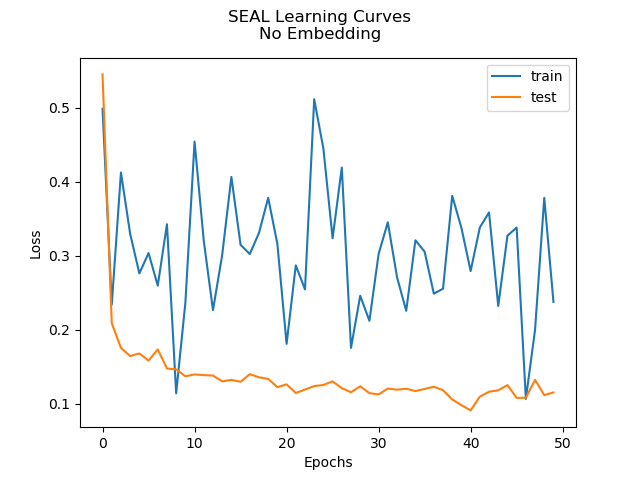
\includegraphics[scale=0.35]{latex/images/No Embedding.png}
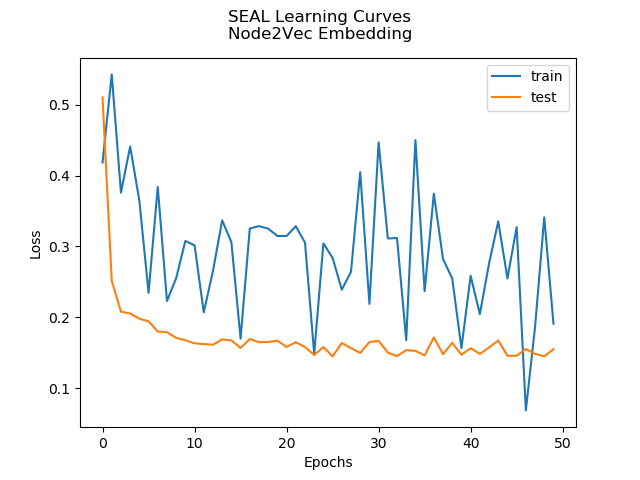
\includegraphics[scale=0.35]{latex/images/Node2Vec Embedding.png}
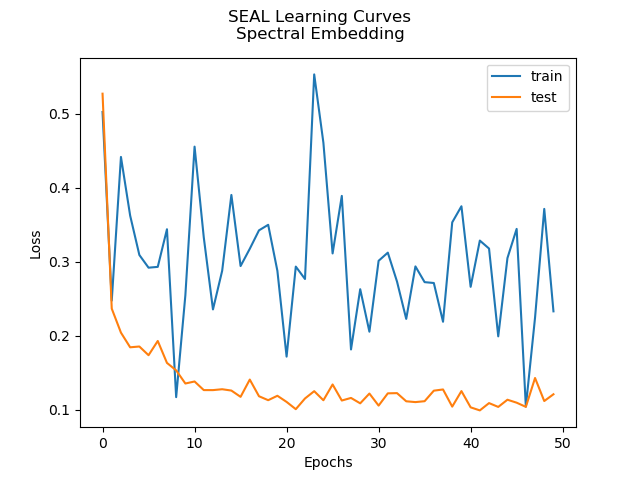
\includegraphics[scale=0.35]{latex/images/Spectral Embedding.png}
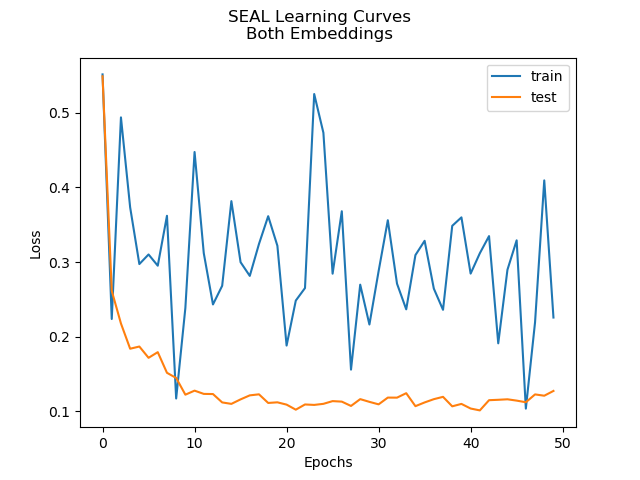
\includegraphics[scale=0.35]{latex/images/Both Embeddings.png}
\end{center}



\begin{table*}
\begin{center}
\begin{tabular}{|l|c|c|c|c|c|}
\hline
SEAL & Time & ROC after 50 epochs  & AP after 50 epochs & Best ROC & Best AP \\
\hline\hline
No Embedding & 312.98s & 0.936 & 0.916 & 0.936 & 0.916\\
Node2Vec & 384.77s & 0.923 & 0.906 & 0.924 & 0.906\\
Spectral  & 360.52s & 0.932 & 0.916 & 0.935 & 0.917\\
Both  & 403.85s & 0.934 & 0.921 & 0.934 & 0.921\\
\hline
\end{tabular}
\end{center}
\caption{Comparisons of different embeddings with SEAL trained on 50 epochs of 3-hop data set.}
\label{tab:contributions}
\end{table*}

\begin{table*}
\begin{center}
\begin{tabular}{|l|c|c|c|c|c|}
\hline
SEAL & Time & ROC after 50 epochs  & AP after 50 epochs & Best ROC & Best AP \\
\hline\hline
No Embedding & 363.96s & 0.936 & 0.919 & 0.936 & 0.919\\
Node2Vec & 461.40s & 0.932 & 0.919 & 0.932 & 0.920\\
Spectral & 428.12s & 0.939 & 0.926 & 0.939 & 0.926\\
Both  & 458.80s & 0.939 & 0.927 & 0.939 & 0.927\\
\hline
\end{tabular}
\end{center}
\caption{Comparisons of different embeddings with SEAL trained on 50 epochs of 5-hop data set.}
\label{tab:contributions}
\end{table*}

\subsection{VGAE - Variational Graph Autoencoders}

As the graph is too large and experiments show that categories are strongly inter-related, we decide to choose top-K nodes with the highest degree and their neighbours so that we can still encode the important information in the graph. For our feature matrix, we only use the following attributes - 'age', 'length', 'views', 'rate', 'rating', 'comments'. For our experiments below we report the ROC-AUC score and the Average-Precision score which can be defined as the area under the area under the receiver operating characteristic curve and the area under the precision-recall curve respectively. \\
We first run an experiment taking the top 1000 nodes with highest degree and varying the number of related videos considered. The results are as follows -  

\begin{center}
\begin{tabular}{|c|c|c|}
\hline
Number of related videos & ROC-AUC Score & AP Score \\
\hline\hline
20 & 0.816 & 0.793\\
15 & 0.802 & 0.777 \\
10 & 0.761 & 0.740 \\
\hline
\end{tabular}
\end{center}
We then also decided to take the top 1000 viewed and rated videos and see if these subsets perform any better. We observed that - 

\begin{center}
\begin{tabular}{|c|c|c|}
\hline
 & ROC-AUC Score & AP Score \\
\hline\hline
Top 1000 viewed videos & 0.787 & 0.775\\
Top 1000 rated videos & 0.827 & 0.809 \\
\hline
\end{tabular}
\end{center}
We can therefore conclude that we want to use the highly rated videos and all the twenty related videos to make better predictions. We can train on more nodes by using a GPU.

\section{Conclusion}

In conclusion, we were able to show that given a dataset that could be represented and shown as a network through the use of the related IDs field, representation learning algorithms / embeddings in combination with a GNN yielded surprisingly strong results. Based on the results that we gathered prior to running the GNN, we conclude that the feature learning process was crucial for high performance and accuracy. After running the GNNs, we observe that the features that are used in heavily impact the model's performance, whether they are learned like with the Variational Graph Autoencoders or explicitly pre-computed as in SEAL.

The work here demonstrates that given an accurate representation of a network, graph neural networks could be a practical application - especially so for non-linear dimensional data sets.

Future work could also involve the use of other well-known, high heuristic order algorithms such as PageRank (used by Google for representation learning on pages on the WorldWide Web) and the Katz index. 

\section{Work Division}

Our work delegation of work among team members can be seen at Table \ref{tab:contributions}.


\begin{table*}
\begin{left}
\begin{tabular}{|l|c|c|}
\hline
Student Name & Contributed Aspects & Details \\
\hline\hline
David Gong & Writing, implementation, article research & Implemented / analyzed link prediction algorithms + spectral embedding \\
Reagan Kan & Writing, implementation, article research & Parse/split data set. Add spectral embedding to SEAL + analyzed results. \\
Sreyans Sipani & Writing, implementation and research & Researched+implemented+experimented-variational graph auto-encoder \\
Jeremy Kwok & & \\
\hline
\end{tabular}
\end{left}
\caption{Contributions of team members.}
\label{tab:contributions}
\end{table*}

% \section{Experiments and Results (MOVED TO SECTION 6)}

% \textbf{(10 points) How did you measure success? What experiments were used? What were the results, both quantitative and qualitative? Did you succeed? Did you fail? Why? Justify your reasons with arguments supported by evidence and data.}

% Our results were as follows

% \textbf{Important: This section should be rigorous and thorough. Present detailed information about decision you made, why you made them, and any evidence/experimentation to back them up. This is especially true if you leveraged existing architectures, pre-trained models, and code (i.e. do not just show results of fine-tuning a pre-trained model without any analysis, claims/evidence, and conclusions, as that tends to not make a strong project). }

%-------------------------------------------------------------------------
% \section{Other Sections}

% You are welcome to introduce additional sections or subsections, if required, to address the following questions in detail. 

% (5 points) Appropriate use of figures / tables / visualizations. Are the ideas presented with appropriate illustration? Are the results presented clearly; are the important differences illustrated? 

% (5 points) Overall clarity. Is the manuscript self-contained? Can a peer who has also taken Deep Learning understand all of the points addressed above? Is sufficient detail provided? 

% (5 points) Finally, points will be distributed based on your understanding of how your project relates to Deep Learning. Here are some questions to think about: 

% What was the structure of your problem? How did the structure of your model reflect the structure of your problem? 

% What parts of your model had learned parameters (e.g., convolution layers) and what parts did not (e.g., post-processing classifier probabilities into decisions)? 

% What representations of input and output did the neural network expect? How was the data pre/post-processed?
% What was the loss function? 

% Did the model overfit? How well did the approach generalize? 

% What hyperparameters did the model have? How were they chosen? How did they affect performance? What optimizer was used? 

% What Deep Learning framework did you use? 

% What existing code or models did you start with and what did those starting points provide? 

% Briefly discuss potential future work that the research community could focus on to make improvements in the direction of your project's topic.


% %-------------------------------------------------------------------------
% \section{Miscellaneous Information}

% The rest of the information in this format template has been adapted from CVPR 2020 and provides guidelines on the lower-level specifications regarding the paper's format.

% \subsection{Language}

% All manuscripts must be in English.

% \subsection{Dual submission}

% Please refer to the author guidelines on the CVPR 2020 web page for a
% discussion of the policy on dual submissions.

% \subsection{Paper length}
% Papers, excluding the references section,
% must be no longer than eight pages in length. The references section
% will not be included in the page count, and there is no limit on the
% length of the references section. For example, a paper of eight pages
% with two pages of references would have a total length of 10 pages.
% {\bf There will be no extra page charges for CVPR 2020.}

% Overlength papers will simply not be reviewed.  This includes papers
% where the margins and formatting are deemed to have been significantly
% altered from those laid down by this style guide.  Note that this
% \LaTeX\ guide already sets figure captions and references in a smaller font.
% The reason such papers will not be reviewed is that there is no provision for
% supervised revisions of manuscripts.  The reviewing process cannot determine
% the suitability of the paper for presentation in eight pages if it is
% reviewed in eleven.  

% %-------------------------------------------------------------------------
% \subsection{The ruler}
% The \LaTeX\ style defines a printed ruler which should be present in the
% version submitted for review.  The ruler is provided in order that
% reviewers may comment on particular lines in the paper without
% circumlocution.  If you are preparing a document using a non-\LaTeX\
% document preparation system, please arrange for an equivalent ruler to
% appear on the final output pages.  The presence or absence of the ruler
% should not change the appearance of any other content on the page.  The
% camera ready copy should not contain a ruler. (\LaTeX\ users may uncomment
% the \verb'\cvprfinalcopy' command in the document preamble.)  Reviewers:
% note that the ruler measurements do not align well with lines in the paper
% --- this turns out to be very difficult to do well when the paper contains
% many figures and equations, and, when done, looks ugly.  Just use fractional
% references (e.g.\ this line is $095.5$), although in most cases one would
% expect that the approximate location will be adequate.

% \subsection{Mathematics}

% Please number all of your sections and displayed equations.  It is
% important for readers to be able to refer to any particular equation.  Just
% because you didn't refer to it in the text doesn't mean some future reader
% might not need to refer to it.  It is cumbersome to have to use
% circumlocutions like ``the equation second from the top of page 3 column
% 1''.  (Note that the ruler will not be present in the final copy, so is not
% an alternative to equation numbers).  All authors will benefit from reading
% Mermin's description of how to write mathematics:
% \url{http://www.pamitc.org/documents/mermin.pdf}.

% Finally, you may feel you need to tell the reader that more details can be
% found elsewhere, and refer them to a technical report.  For conference
% submissions, the paper must stand on its own, and not {\em require} the
% reviewer to go to a techreport for further details.  Thus, you may say in
% the body of the paper ``further details may be found
% in~\cite{Authors14b}''.  Then submit the techreport as additional material.
% Again, you may not assume the reviewers will read this material.

% Sometimes your paper is about a problem which you tested using a tool which
% is widely known to be restricted to a single institution.  For example,
% let's say it's 1969, you have solved a key problem on the Apollo lander,
% and you believe that the CVPR70 audience would like to hear about your
% solution.  The work is a development of your celebrated 1968 paper entitled
% ``Zero-g frobnication: How being the only people in the world with access to
% the Apollo lander source code makes us a wow at parties'', by Zeus \etal.

% You can handle this paper like any other.  Don't write ``We show how to
% improve our previous work [Anonymous, 1968].  This time we tested the
% algorithm on a lunar lander [name of lander removed for blind review]''.
% That would be silly, and would immediately identify the authors. Instead
% write the following:
% \begin{quotation}
% \noindent
%   We describe a system for zero-g frobnication.  This
%   system is new because it handles the following cases:
%   A, B.  Previous systems [Zeus et al. 1968] didn't
%   handle case B properly.  Ours handles it by including
%   a foo term in the bar integral.

%   ...

%   The proposed system was integrated with the Apollo
%   lunar lander, and went all the way to the moon, don't
%   you know.  It displayed the following behaviours
%   which show how well we solved cases A and B: ...
% \end{quotation}
% As you can see, the above text follows standard scientific convention,
% reads better than the first version, and does not explicitly name you as
% the authors.  A reviewer might think it likely that the new paper was
% written by Zeus \etal, but cannot make any decision based on that guess.
% He or she would have to be sure that no other authors could have been
% contracted to solve problem B.
% \medskip

% \noindent
% FAQ\medskip\\
% {\bf Q:} Are acknowledgements OK?\\
% {\bf A:} No.  Leave them for the final copy.\medskip\\
% {\bf Q:} How do I cite my results reported in open challenges?
% {\bf A:} To conform with the double blind review policy, you can report results of other challenge participants together with your results in your paper. For your results, however, you should not identify yourself and should not mention your participation in the challenge. Instead present your results referring to the method proposed in your paper and draw conclusions based on the experimental comparison to other results.\medskip\\

% \begin{figure}[t]
% \begin{center}
% \fbox{\rule{0pt}{2in} \rule{0.9\linewidth}{0pt}}
%   %\includegraphics[width=0.8\linewidth]{egfigure.eps}
% \end{center}
%   \caption{Example of caption.  It is set in Roman so that mathematics
%   (always set in Roman: $B \sin A = A \sin B$) may be included without an
%   ugly clash.}
% \label{fig:long}
% \label{fig:onecol}
% \end{figure}

% \subsection{Miscellaneous}

% \noindent
% Compare the following:\\
% \begin{tabular}{ll}
%  \verb'$conf_a$' &  $conf_a$ \\
%  \verb'$\mathit{conf}_a$' & $\mathit{conf}_a$
% \end{tabular}\\
% See The \TeX book, p165.

% The space after \eg, meaning ``for example'', should not be a
% sentence-ending space. So \eg is correct, {\em e.g.} is not.  The provided
% \verb'\eg' macro takes care of this.

% When citing a multi-author paper, you may save space by using ``et alia'',
% shortened to ``\etal'' (not ``{\em et.\ al.}'' as ``{\em et}'' is a complete word.)
% However, use it only when there are three or more authors.  Thus, the
% following is correct: ``
%   Frobnication has been trendy lately.
%   It was introduced by Alpher~\cite{4539688}, and subsequently developed by
%   Alpher and Fotheringham-Smythe~\cite{zhang2018link}, and Alpher \etal~\cite{Alpher04}.''

% This is incorrect: ``... subsequently developed by Alpher \etal~\cite{Alpher03} ...''
% because reference~\cite{Alpher03} has just two authors.  If you use the
% \verb'\etal' macro provided, then you need not worry about double periods
% when used at the end of a sentence as in Alpher \etal.

% For this citation style, keep multiple citations in numerical (not
% chronological) order, so prefer \cite{Alpher03,Alpher02,Authors14} to
% \cite{Alpher02,Alpher03,Authors14}.


% \begin{figure*}
% \begin{center}
% \fbox{\rule{0pt}{2in} \rule{.9\linewidth}{0pt}}
% \end{center}
%   \caption{Example of a short caption, which should be centered.}
% \label{fig:short}
% \end{figure*}

% %------------------------------------------------------------------------
% \subsection{Formatting your paper}

% All text must be in a two-column format. The total allowable width of the
% text area is $6\frac78$ inches (17.5 cm) wide by $8\frac78$ inches (22.54
% cm) high. Columns are to be $3\frac14$ inches (8.25 cm) wide, with a
% $\frac{5}{16}$ inch (0.8 cm) space between them. The main title (on the
% first page) should begin 1.0 inch (2.54 cm) from the top edge of the
% page. The second and following pages should begin 1.0 inch (2.54 cm) from
% the top edge. On all pages, the bottom margin should be 1-1/8 inches (2.86
% cm) from the bottom edge of the page for $8.5 \times 11$-inch paper; for A4
% paper, approximately 1-5/8 inches (4.13 cm) from the bottom edge of the
% page.

% %-------------------------------------------------------------------------
% \subsection{Margins and page numbering}

% All printed material, including text, illustrations, and charts, must be kept
% within a print area 6-7/8 inches (17.5 cm) wide by 8-7/8 inches (22.54 cm)
% high.



% %-------------------------------------------------------------------------
% \subsection{Type-style and fonts}

% Wherever Times is specified, Times Roman may also be used. If neither is
% available on your word processor, please use the font closest in
% appearance to Times to which you have access.

% MAIN TITLE. Center the title 1-3/8 inches (3.49 cm) from the top edge of
% the first page. The title should be in Times 14-point, boldface type.
% Capitalize the first letter of nouns, pronouns, verbs, adjectives, and
% adverbs; do not capitalize articles, coordinate conjunctions, or
% prepositions (unless the title begins with such a word). Leave two blank
% lines after the title.

% AUTHOR NAME(s) and AFFILIATION(s) are to be centered beneath the title
% and printed in Times 12-point, non-boldface type. This information is to
% be followed by two blank lines.

% The ABSTRACT and MAIN TEXT are to be in a two-column format.

% MAIN TEXT. Type main text in 10-point Times, single-spaced. Do NOT use
% double-spacing. All paragraphs should be indented 1 pica (approx. 1/6
% inch or 0.422 cm). Make sure your text is fully justified---that is,
% flush left and flush right. Please do not place any additional blank
% lines between paragraphs.

% Figure and table captions should be 9-point Roman type as in
% Figures~\ref{fig:onecol} and~\ref{fig:short}.  Short captions should be centred.

% \noindent Callouts should be 9-point Helvetica, non-boldface type.
% Initially capitalize only the first word of section titles and first-,
% second-, and third-order headings.

% FIRST-ORDER HEADINGS. (For example, {\large \bf 1. Introduction})
% should be Times 12-point boldface, initially capitalized, flush left,
% with one blank line before, and one blank line after.

% SECOND-ORDER HEADINGS. (For example, { \bf 1.1. Database elements})
% should be Times 11-point boldface, initially capitalized, flush left,
% with one blank line before, and one after. If you require a third-order
% heading (we discourage it), use 10-point Times, boldface, initially
% capitalized, flush left, preceded by one blank line, followed by a period
% and your text on the same line.

% %-------------------------------------------------------------------------
% \subsection{Footnotes}

% Please use footnotes\footnote {This is what a footnote looks like.  It
% often distracts the reader from the main flow of the argument.} sparingly.
% Indeed, try to avoid footnotes altogether and include necessary peripheral
% observations in
% the text (within parentheses, if you prefer, as in this sentence).  If you
% wish to use a footnote, place it at the bottom of the column on the page on
% which it is referenced. Use Times 8-point type, single-spaced.


%-------------------------------------------------------------------------
% \subsection{References}

% List and number all bibliographical references in 9-point Times,
% single-spaced, at the end of your paper. When referenced in the text,
% enclose the citation number in square brackets, for
% example~\cite{Authors14}.  Where appropriate, include the name(s) of
% editors of referenced books.


% \begin{table}
% \begin{center}
% \begin{tabular}{|l|c|}
% \hline
% Method & Frobnability \\
% \hline\hline
% Theirs & Frumpy \\
% Yours & Frobbly \\
% Ours & Makes one's heart Frob\\
% \hline
% \end{tabular}
% \end{center}
% \caption{Results.   Ours is better.}
% \end{table}

% %-------------------------------------------------------------------------
% \subsection{Illustrations, graphs, and photographs}

% All graphics should be centered.  Please ensure that any point you wish to
% make is resolvable in a printed copy of the paper.  Resize fonts in figures
% to match the font in the body text, and choose line widths which render
% effectively in print.  Many readers (and reviewers), even of an electronic
% copy, will choose to print your paper in order to read it.  You cannot
% insist that they do otherwise, and therefore must not assume that they can
% zoom in to see tiny details on a graphic.

% When placing figures in \LaTeX, it's almost always best to use
% \verb+\includegraphics+, and to specify the  figure width as a multiple of
% the line width as in the example below
% {\small\begin{verbatim}
%   \usepackage[dvips]{graphicx} ...
%   \includegraphics[width=0.8\linewidth]
%                   {myfile.eps}
% \end{verbatim}
% }


% %-------------------------------------------------------------------------
% \subsection{Color}

% Please refer to the author guidelines on the CVPR 2020 web page for a discussion
% of the use of color in your document.

%------------------------------------------------------------------------

%-------------------------------------------------------------------------



{\small
\bibliographystyle{ieee_fullname}
\bibliography{egbib}
}

\end{document}
